\documentclass[conference]{IEEEtran}

\usepackage{cite}
\usepackage{subfig}
\usepackage{amsmath,amssymb,amsfonts}
\usepackage{algorithmic}
\usepackage{graphicx}
\usepackage{textcomp}
\usepackage{xcolor}
\usepackage{float}
\usepackage{booktabs}
\usepackage{pxfonts}
\usepackage{listings}
\usepackage{epstopdf}
\usepackage{import}


\def\BibTeX{{\rm B\kern-.05em{\sc i\kern-.025em b}\kern-.08em
    T\kern-.1667em\lower.7ex\hbox{E}\kern-.125emX}}

% Define standard verbatim listing style
\lstdefinestyle{standard}{
  basicstyle=\fontsize{9}{9}\ttfamily,
  columns=flexible,
  breaklines=true,
  escapechar=\#
}

\newcommand\inputpgf[2]{{
\let\pgfimageWithoutPath\pgfimage
\renewcommand{\pgfimage}[2][]{\pgfimageWithoutPath[##1]{#1/##2}}
\input{#1/#2}
}}

\usepackage{tikz}
\usepackage{pgfplots}

\newcommand{\mytilde}{\raise.17ex\hbox{$\scriptstyle\mathtt{\sim}$}}


\begin{document}
\title{Biometrics: Body Shape Recognition\\
}

\author{\IEEEauthorblockN{\textbf{David Jones}}
\IEEEauthorblockA{\textit{School of Electronics and Computer Science} \\
\textit{University of Southampton}\\
Southampton, United Kingdom \\
dsj1n15@ecs.soton.ac.uk}
}
\maketitle

\begin{abstract}
  The role of a biometric system is to identify subjects for purposes including access control and authentication. This report studies the use of body-shape features as a means to classify subjects. The approach taken utilises state-of-the-art neural networks for pose estimation and semantic segmentation before applying more traditional techniques to define feature vectors. The approach has a CCR of 91\% and EER of 33\%. Increasing performance was largely handicapped by the irregularities in the small dataset and lack of subject repetition.
\end{abstract}

\begin{IEEEkeywords}
Identification, Body Shape, Limb, Shape Descriptors, Pose Estimation, Semantic Segmentation
\end{IEEEkeywords}

\section{Introduction}
\noindent A requirement for a biometric system is being able to to differentiate subjects. Existing image based systems typically use facial recognition \cite{biometric_systems}, whereas video systems may aim to categorise people's gait \cite{Nixon_Tan_Chellappa_2006}. This report identifies the feasibility of body-shape features on a small image dataset with side-on and front-on views of each subject. A second dataset with some subjects repeated is then then used to assess classification performance. Datasets are subsets of the Large Southampton Gait Database \cite{shutler:gait_database} (Figure \ref{fig:dataset_examples}).

\begin{figure}[H]
  \centering
  \begin{tabular}{cc}
  \subfloat[Front]{
  \begin{tabular}{c}
    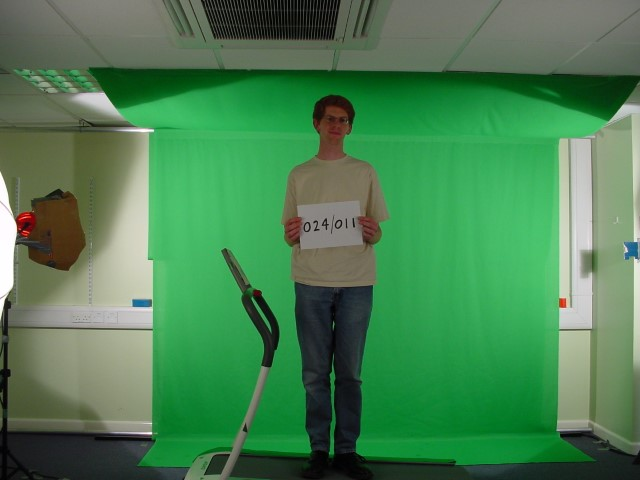
\includegraphics[width=0.22\textwidth]{figures/024z011pf.jpg}\\
    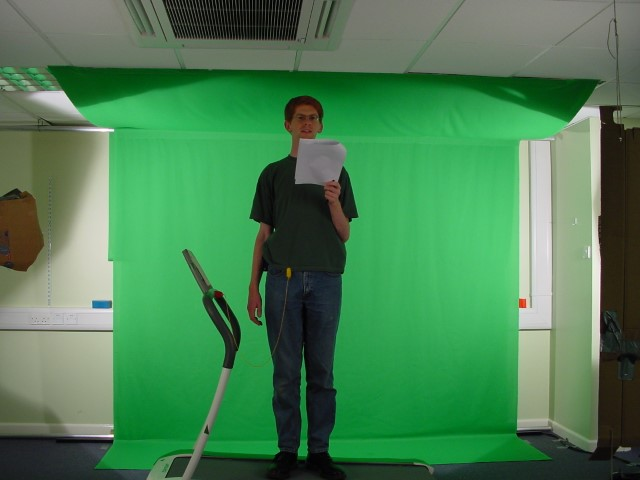
\includegraphics[width=0.22\textwidth]{figures/DSC00185.jpg}
  \end{tabular}
  }
  \hspace{-6mm}
  \subfloat[Side]{
  \begin{tabular}{c}
    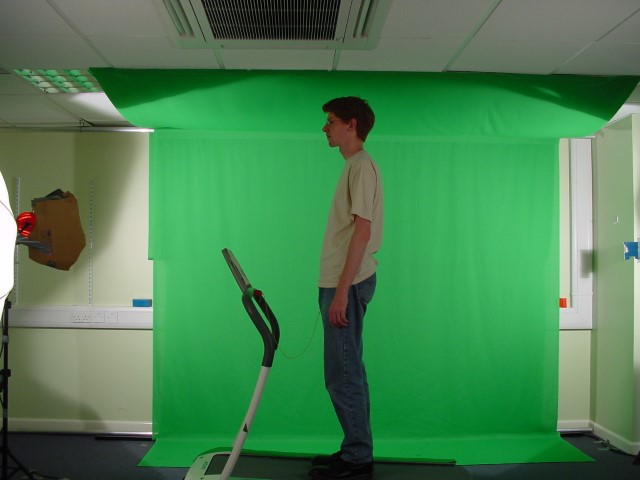
\includegraphics[width=0.22\textwidth]{figures/024z011ps.jpg}\\
    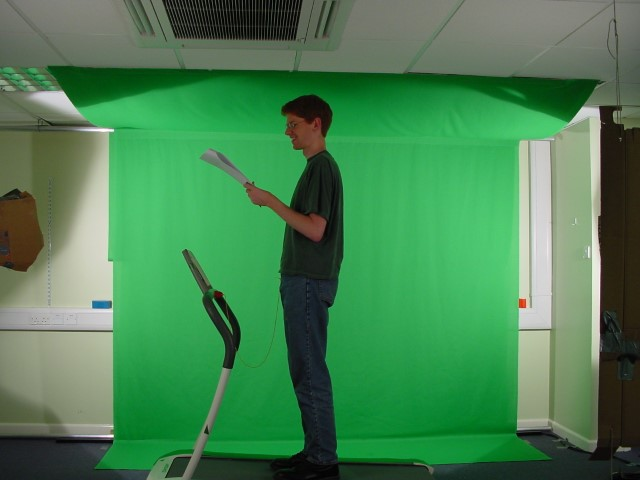
\includegraphics[width=0.22\textwidth]{figures/DSC00186.jpg}
  \end{tabular}
  }
  \end{tabular}
  \caption{Example of subject present in both datasets.}
  \label{fig:dataset_examples}
\end{figure}

\section{Method}
\noindent This section details feature-vector generation and classification methods. In addition to those mentioned, the Python implementation utilised the common libraries: NumPy\footnote{Numpy, https://numpy.org/} OpenCV\footnote{OpenCV, https://opencv.org/} , PyTorch\footnote{PyTorch, https://pytorch.org/} and SKLearn\footnote{scikit learn, https://scikit-learn.org/},


\subsection{Features}
\noindent The final feature-vectors are made from a selection of measurements and moments; those used depend on the view. Images were resized to have a height of 600px whilst keeping the same aspect ratio to reduce computation.\\

\subsubsection{Subject Mask}
The first stage of feature extraction was to find which pixels of the input belong to the subject; this is referred to as image segmentation. The subject mask was generated in two stages: 
\begin{enumerate}
  \item Semantic segmentation performed by a Convolutional Neural Network (CNN), specifically DeepLabV3 ResNet101 \cite{DBLP:journals/corr/ChenPSA17}. Torchvision's\footnote{Torchvision, https://pytorch.org/docs/stable/)torchvision} implementation was used.
  \item This did not follow the body contours completely (Figure \ref{fig:sem_seg}), so a further green-screen removal stage was done in the HSV colour space. (Figure \ref{fig:final_seg})
\end{enumerate}


\begin{figure}[H]
  \centering
  \begin{tabular}{cccc}
  \subfloat[]{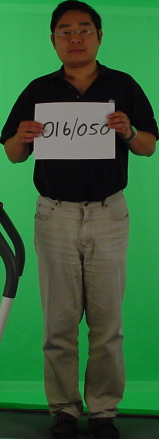
\includegraphics[width=0.10\textwidth]{figures/mask_input.png}}
  \hspace{1.5mm}
  \subfloat[\label{fig:sem_seg}]{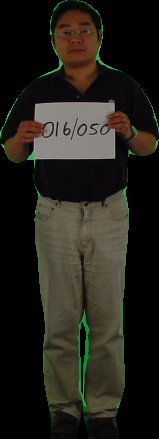
\includegraphics[width=0.10\textwidth]{figures/mask_semantic.png}}
  \hspace{1.5mm}
  \subfloat[\label{fig:final_seg}]{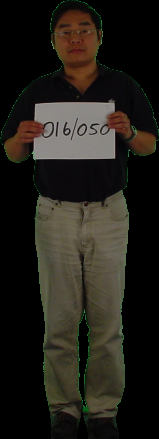
\includegraphics[width=0.10\textwidth]{figures/mask_final.png}}
  \hspace{1.5mm}
  \subfloat[]{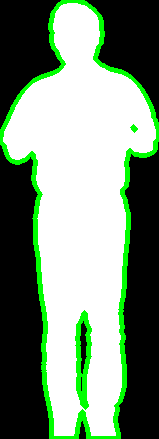
\includegraphics[width=0.10\textwidth]{figures/mask_contour.png}}
  \end{tabular}
  \caption{Masking example: input, semanticly segemented, green screen removed, silhouette with extracted contour points (left--right). Note that the example images are cropped, the actual system accepts full images.}
\end{figure}


\noindent This method lead to perfect mask generation for all subjects. Traditional methods including active contours typically failed where there was crossover with the treadmill.\\

\noindent \textit{Hu Moments} were generated from the full-body mask to form part of the feature vector for the side-on views. These are preferable to area/perimeter as they are invariant to translation, scale and rotation. A \textit{height} metric was also calculated by finding the difference between the lower and upper bounds of the mask. \\

\subsubsection{Keypoint Estimation}
 Fitting a virtual skeleton to a body is known as pose estimation. This method identifies body keypoints with understanding of the underlying semantics that dictate their position; this allows extraction where limbs are occluded or overlap. Torchvision's implementation of Keypoint R-CNN \cite{he2017mask} was used to extract 17 XY keypoints. These were reordered and an extra keypoint was extrapolated for the chest to match OpenPose's\footnote{OpenPose, https://git.io/JfVsu} data format (Figure \ref{fig:poses}).

\begin{figure}[H]
  \centering
  \begin{tabular}{cc}
  \subfloat[]{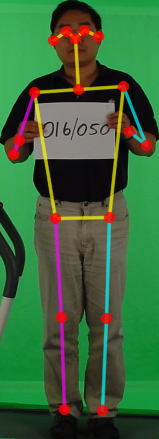
\includegraphics[height=2.3in]{figures/front_kp_a.png} 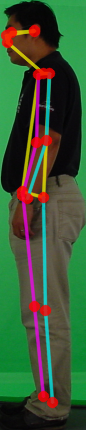
\includegraphics[height=2.3in]{figures/side_kp_a.png}}
  \hspace{1.5mm}
  \subfloat[]{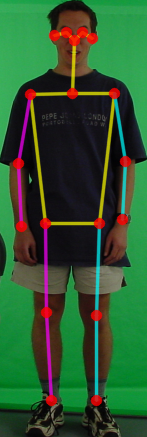
\includegraphics[height=2.3in]{figures/front_kp_b.png} 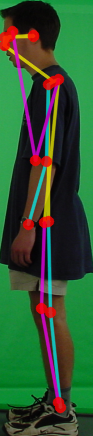
\includegraphics[height=2.3in]{figures/side_kp_b.png}}
  \end{tabular}
  \caption{Keypoint estimation on two subjects.}\label{fig:poses}
\end{figure}

\noindent These keypoints were accurate where positioning was not subjective, e.g. for noses, but not always where many positions would be acceptable e.g. the pelvis. Additionally because Z data is not estimated, distances between points cannot take into account depth. Points were therefore mostly used to orientate other features. However, where distances were relatively consistent it was possible to add them to the feature vector; those used are labelled in Figure \ref{fig:measurements}. It would be preferable if these measurements were scale invariant in case the subject stood a different distance from the camera but attempting to normalise off one measurement made the features highly non-differentiable.

\begin{figure}[H]
  \centering
  \begin{tabular}{cc}
  \subfloat[]{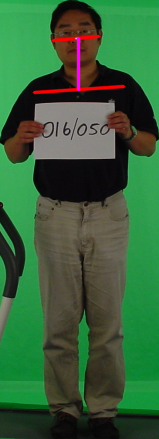
\includegraphics[height=2.3in]{figures/front_measurements_a.png} 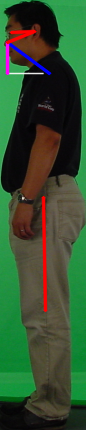
\includegraphics[height=2.3in]{figures/side_measurements_a.png}}
  \hspace{1.5mm}
  \subfloat[]{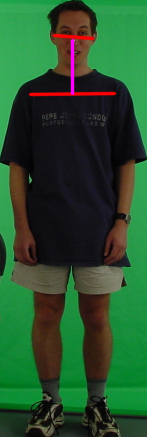
\includegraphics[height=2.3in]{figures/front_measurements_b.png} 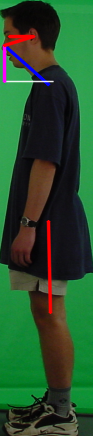
\includegraphics[height=2.3in]{figures/side_measurements_b.png}}
  \end{tabular}
  \caption{Keypoint measurements for each view. red, pink, blue lines indicate where Euclidain distance, Y Manhatten distance and angle (from the horizontal) are used respectively.}\label{fig:measurements}
\end{figure}



\subsubsection{Head Mask Extraction}
Some subjects have different clothes between the validation and testsets; this reduces effectiveness of the full-body mask. Extracting the head portion provides a more consistent shape.

\begin{figure}[H]
  \centering
  \begin{tabular}{cc}
  \subfloat[]{
\includegraphics[height=0.75in]{figures/front_head_a.png} 
\includegraphics[height=0.75in]{figures/side_head_a.png}}
  \hspace{1.5mm}&
  \subfloat[]{
\includegraphics[height=0.75in]{figures/front_head_b.png} 
\includegraphics[height=0.75in]{figures/side_head_b.png}}\\
  \vspace{1.5mm}
  \subfloat[]{
\includegraphics[height=0.75in]{figures/front_head_c.png} 
\includegraphics[height=0.75in]{figures/side_head_c.png}}
  \hspace{1.5mm}&
  \subfloat[]{
\includegraphics[height=0.75in]{figures/front_head_d.png} 
\includegraphics[height=0.75in]{figures/side_head_d.png}}
  \end{tabular}
  \caption{Example head masks (front--side for each subject).}
\end{figure}

\noindent There are no keypoints to make neck extraction straightforward. Simple methods may attempt to find the thinnest point of the mask however this fails with hair and does not take into account the angle of the neck for the side-on view. The following method was used:
\begin{enumerate}
  \item Extract the contour of the full-body.
  \item Trace from the shoulder keypoints to the edge of the contour on the left/right (side-on) and top (front-on) to find two starting points.
  \item Plot the X positions following the contour upwards.
  \item Use peak/trough detection to find the turning points (where the head begins).
  \item Remove proceeding points of the contour to create a contour of just the head.
  \item Convert this contour to a mask.
\end{enumerate}
Performing this process results in near-perfect head extractions on which \textit{Hu Moments} are generated for all views.


\subsection{Classifier}
\noindent The classifier expects both front-on and side-on views of a subject where the view is inferred as part of feature extraction. The different views use different feature vectors so cannot be directly compared. To this end separate k-nearest-neighbour classifiers are used for each view -- $k=1$ due to lack of repetition in the dataset. These are trained on the \textit{authorised} user set with feature normalisation applied to keep the subject distances between 0 and \mytilde 1. These are combined by taking the mean of the all distance vectors generated; this allows classification via further views or repetitions of the same view. A threshold calculated via the EER is applied to limit false classifications. SVMs were considered, however reduced relevance of the easily comparable distance metric and lack of advantages due to the small dataset meant k-NN was preferable.
\section{Results}
\noindent To assess the system the \texttt{test} dataset (11 classes) were treated as the \textit{authorised} subjects, whereas the \texttt{train} dataset (44 classes) were treated as the \textit{input} subjects. The resultant Euclidean distances between feature vectors are shown in Figure \ref{fig:feature_distances}.

\begin{figure}[H]
  \centering
  \begin{tabular}{c}
  \subfloat[Front-On]{\inputpgf{figures/}{front_distances.pgf}}\\
  \subfloat[Side-On]{\inputpgf{figures/}{side_distances.pgf}}\\
  \subfloat[Combined]{\inputpgf{figures/}{combined_distances.pgf}}
  \end{tabular}
  \caption{Log Euclidean distances between subjects. Each row represents an \textit{authorised} subject against all \textit{inputs}. See Figure \ref{fig:ccr_plot} for correct classifications.}\label{fig:feature_distances}
\end{figure}


\noindent The side-on and front-on classifiers can both be tuned to achieve 63\% CCR individually, however a focus is placed on assessment of the combined system. Metrics were calculated as:
\begin{itemize}
  \item \textbf{CCR:} Correct Recognition Rate -- Percentage of \textit{input} subjects who were closest to their corresponding \textit{authorised} subject.
  \item \textbf{T-CCR:} Threshold-CCR -- CCR but taking into account threshold calculated via EER.
  \item \textbf{FAR:} False Accept Rate -- Percentage of \textit{input} subjects not in the \textit{authorised} dataset who were within the allowed threshold of an \textit{authorised} subject.
  \item \textbf{FRR:} False Reject Rate -- Percentage of \textit{input} subjects who were not within the threshold of their corresponding \textit{authorised} subject.
\end{itemize}

\noindent The EER of 33\% was calculated from the intersect of the FAR and FRR (Figure \ref{fig:eer_plot}), yielding a threshold distance of 0.15. Figure \ref{fig:ccr_plot} shows the accuracy of the system is 91\% (10/11), reduced to 64\% when thresholding (7/11).

\begin{figure}[H]\centering
  \inputpgf{figures/}{eer_plot.pgf}
  \caption{EER Plot -- Intercept = (0.15, 0.33)}\label{fig:eer_plot}
\end{figure}



\begin{figure}[H]\centering
  \inputpgf{figures/}{ccr_plot.pgf}
  \caption{T-CCR Plot -- True positives, false negatives and false positives shown by green, orange, red respectively. Note where classified incorrectly, green identifies the correct class.}\label{fig:ccr_plot}
\end{figure}

\subsection{Speed}
\noindent A single recognition took 10.2s running on a CPU (Intel i7 8700K). Much of this time was taken up by the segmentation and keypoint detection performed by neural networks. However, these were integrated with GPU support so when tied with a Nvidia GeForce 1080 Ti this time was 0.6s.
Note that masks/keypoints can be cached for the validation set.

\section{Discussion}

\ref{fig:feature_distances} clearly shows the diagonal pattern between x=23 and x=32 where each input closely matches the target.


It is common for a single extracted feature to perform match badly; this increases the overall distance which leads to the EER threshold having to be increased.

\subsection{Improvements}


\subsection{Considered Approaches}
Gabor Wavelets
Insted of applying nearest neighbour to the feature-vectors, bags of features were made on different neig

There is high varience in feature success. Easy to get one outliers. Attempted multiple feature bags so that they could be weighted or combined based on rank.

Clothes are a big issue for moments front-on, that's why side-on is better
Where possible hu moments were used as they are invarient to scale

\section{Conclusion}
A system has been proposed that is able to classify individuals purely on body-shape. 
Although 
Aim to find 
Future Work: Try on a larger dataset. High varience in the feature success 

Have used neural networks trained off the shelve. If enough data was available training a CNN on the silhouettes may be possible.
\bibliographystyle{IEEEtran}
\bibliography{mybibfile}

%\begin{thebibliography}{00}
%\bibitem{b1} Bluetooth SIG, \textit{``Bluetooth Market Update
%2019''}, White Paper, 2018
%\bibitem{b2} Bluetooth SIG, \textit{``Bluetooth Core Specification
%v5.1''}, White Paper, Bluetooth SIG, 21st January 2019
%\end{thebibliography}
\end{document}